% !TEX root = ../main.tex

\section{New mitigations}

By this point, we have discussed 10 solutions to the multiple withdrawal attack and we evaluated them in terms of compatibility with the standard and attack mitigation (recall the summary in Figure~\ref{tab:comp}). Since none of them precisely satisfy the constraints of ERC20 standard, we now propose two new solutions to mitigate the attack.

% = = = = = = = = = = = = = = = = = = = = = = = = = = = = = = = = = = = = = = = = = = =

\subsection{Proposal 1: Securing \texttt{approve} method}
\label{sec:proposal1}

\begin{figure}[t]
	\centering
	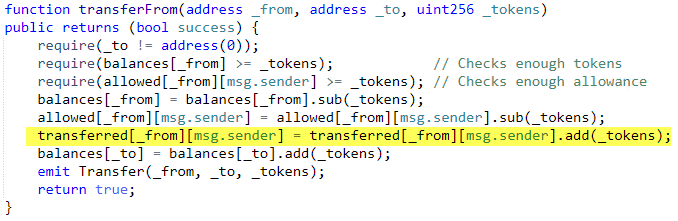
\includegraphics[width=1.0\linewidth]{figures/multiple_withdrawal_14.png}
	\caption{Modified version of \texttt{transferFrom} for keeping track of transferred tokens per spender.\label{fig:transfer1}}
\end{figure}


\begin{figure}[t]
	\centering
	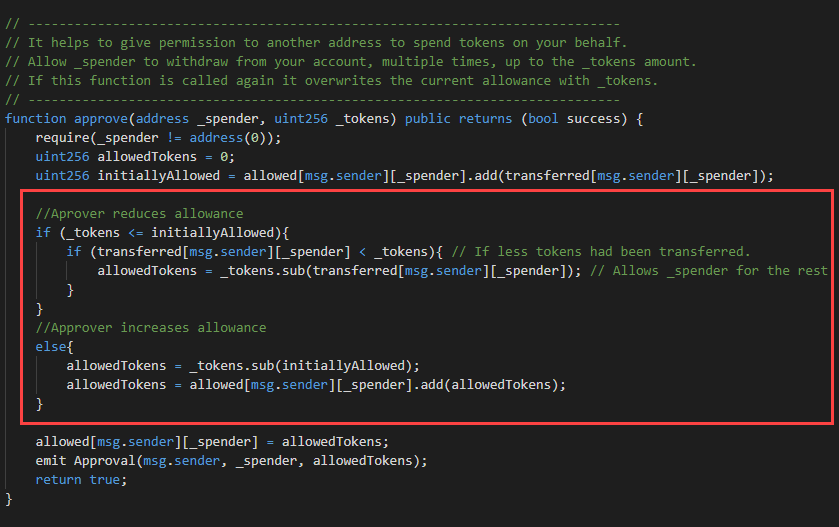
\includegraphics[width=1.0\linewidth]{figures/multiple_withdrawal_15.png}
	\caption{Added code block to \texttt{approve} function to prevent the attack by comparing and setting new allowance atomically.\label{fig:approve1}}
\end{figure}


%Securing \texttt{approve} method could be a solution and prevent the attack. By using compare and set (CAS) pattern \cite{Ref06}, \texttt{approve} method can change spender allowance from N to M atomically (\ie comparing new allowance with transferred token and set it accordingly). Comparison part of CAS requires knowledge of previously transferred tokens that will reveal any token transfer in case of front-running. Although this is promising approach,  setting new allowance in \texttt{approve} method must satisfy ERC20 constraint that dictates "If this function is called again it overwrites the current allowance with \texttt{\_value}" \cite{Ref08}. This does not allow any adjustments in allowance while it is a prerequisite for securing \texttt{approve} method. 

By implementing the CAS pattern~\cite{Ref06} in the \texttt{approve} method, we set up a small state machine so that new allowances can be set atomically after a comparison with transferred tokens. This tracking requires adding a new variable to the \texttt{transferFrom} method (see Figure~\ref{fig:transfer1}). Since this is an internal variable, it is not visible to already deployed smart contracts and keeps the \texttt{transferFrom} function ERC20-compatible. Similarly, a block of code is added to the \texttt{approve} function (see Figure~\ref{fig:approve1}) to work in both cases with zero and non-zero allowances. This new logic in the \texttt{approve} function compares a new allowance---passed as \texttt{\_tokens} argument to the function---with the current allowance of the spender and the already transferred tokens. Allowance are saved in \texttt{allowed[msg.sender][\_spender]} variable as in typical ERC20 implementation, and \texttt{transferred[msg.sender][\_spender]} is the new state. The method decides to increase or decrease the current allowance based on this comparison. If the new allowance is less than initial allowance---sum of \texttt{allowance} and \texttt{transferred} variables---it denotes decreasing of allowance, otherwise increasing of allowance is intended. Such a modified \texttt{approve} function prevents the attack by either increasing or decreasing the allowance instead of setting it to an explicit value.

Unlike other solutions, there is no need to set allowance from N to 0 and then to M. The token holder can directly change the allowance from N to M which saves time waiting for the confirmation of a transaction and any monitoring of the contract. Consider the following transaction sequences to illustrate how the state changes:

% = = = = = = = = = = = = = = = = = = = = = = = = = = = = = = = = = = = = = = = = = = =

\subsubsection*{Scenario A} Alice approves Bob for spending 100 tokens and then decides to increase it to 120 tokens.
\begin{enumerate}
	\item Alice approves Bob for transferring 100 tokens.
	\item After a while, Alice decides to increase Bob’s allowance from 100 to 120 tokens.
	\item Bob noticed Alice’s new transaction and transfers 100 tokens by front-running.
	\item Bob’s allowance is 0 and \texttt{transferred}=100.
	\item Alice’s transaction is mined and checks initial allowance (100) with new allowance (120).
	\item As it is increasing, the new allowance (120) will be subtracted from the transferred tokens (100).
	\item 20 tokens will be set as Bob’s allowance.
	\item Bob would be able to transfer 20 more tokens (120 in total as Alice wanted).\newline
\end{enumerate}
 
\subsubsection*{Scenario B} Alice approves Bob for spending 100 tokens and then decides to decrease it to 10 tokens.
\begin{enumerate}
	\item Alice approves Bob for transferring 100 tokens.
	\item After a while, Alice decides to reduce Bob’s allowance from 100 to 10 tokens.
	\item Bob noticed Alice’s new transaction and transfers 100 tokens by front-running.
	\item Bob’s allowance is 0 and \texttt{transferred}=100 (set by \texttt{transferFrom} function).
	\item Alice’s transaction is mined and checks initial allowance (100) with new allowance (10).
	\item As it is reducing, \texttt{transferred} tokens (100) is compared with new allowance (10). Since Bob already transferred more tokens, his allowance will be set to 0.
	\item Bob is not able to move more than initial 100 approved tokens.
\end{enumerate}

% = = = = = = = = = = = = = = = = = = = = = = = = = = = = = = = = = = = = = = = = = = =

\begin{figure}[t]
	\centering
	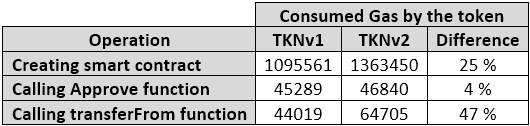
\includegraphics[width=1.0\linewidth]{figures/multiple_withdrawal_22.png}
	\caption{Comparison of gas consumption between standard implementation of ERC20 token (TKNv1) and secured version of it (TKNv2).\label{fig:gas}}
\end{figure}

\subsubsection*{Performance} In order to evaluate functionality of the new \texttt{approve} and \texttt{transferFrom} functions, we have implemented a standard ERC20 token (TKNv1\footnote{https://rinkeby.etherscan.io/address/0x8825bac68a3f6939c296a40f c8078d18c2f66ac7}) along side the proposed ERC20 token (TKNv2\footnote{https://rinkeby.etherscan.io/address/0xf2b34125223ee54dff48f715 67d4b2a4a0c9858b}) on the Rinkeby test network. Our testing for different input values shows that TKNv2 can address \textit{``multiple withdrawal attack''} by making front-running gains ineffective. Moreover, we compared these two tokens in term of gas consumption. TKNv2.\texttt{approve} function uses almost the same amount of gas as TKNv1.\texttt{approve}, however, gas consumption of TKNv2.\texttt{transferFrom} is around 47\% more than TKNv1.\texttt{transferFrom} (see Figure~\ref{fig:gas}). This difference in TKNv2 is because of maintaining a new mapping variable for tracking transferred tokens. In term of compatibility, both are equivalent interoperable with standard wallets (\eg MetaMask) and have not raised any transfer issues.

\subsubsection*{Discussion} In summary, we can use the CAS pattern to implement a secure \texttt{approve} method that can mitigate the attack effectively. However, it violates one of the ERC20 specifications that says: ``If \texttt{approve} function is called again, it overwrites the current allowance with \texttt{\_value}" (item 2 in Section~\ref{sec:criteria}). Our solution does not comply with this as the resulting allowance can be different than what is passed by the approver (as shown in the scenarios above).

Furthermore we argue that is in fact impossible to secure the \texttt{approve} method without adjusting the allowance. Considering the following transaction sequence:

\begin{enumerate}
	\item Alice decides to change Bob's allowance from N to M (M $\leq$ N in this example).
	\item Bob transfers N tokens by front-running and the \texttt{transferred} variable sets to N.
	\item Alice's transaction is mined and the \texttt{approve} method detects Bob's token transfer.
	\item If \texttt{approve} method does not adjust the allowance based on transferred tokens, it has to set it to M---to conform with the standard---which is allowing Bob to transfer more M tokens, or it could fail which deadlocks Bob from future approvals\footnote{Consider Alice wants to allow Bob for transferring M more tokens in addition to initial N tokens (N+M tokens in total). So, she passes M+N to the \texttt{Approve} method. Even in case of front-running by Bob, the \texttt{Approve} method should not throw an exception. Because this is a legitimate withdraw and already approved by Alice. Additionally, there would not be a way of detecting front-running in \texttt{Approve} method. It sees only transferred token without knowledge of their previous value.}.
\end{enumerate}

Therefore the \texttt{approve} method has to adjust the allowance according to transferred tokens, not based on passed input values to the \texttt{approve} method. Overall, there seems to be no solution to secure the \texttt{approve} method while adhering specification of ERC20 standard.

% = = = = = = = = = = = = = = = = = = = = = = = = = = = = = = = = = = = = = = = = = = =


\subsection{Proposal 2: Securing \texttt{transferFrom}}\label{sec:proposal2}

\begin{figure}[t]
	\centering
	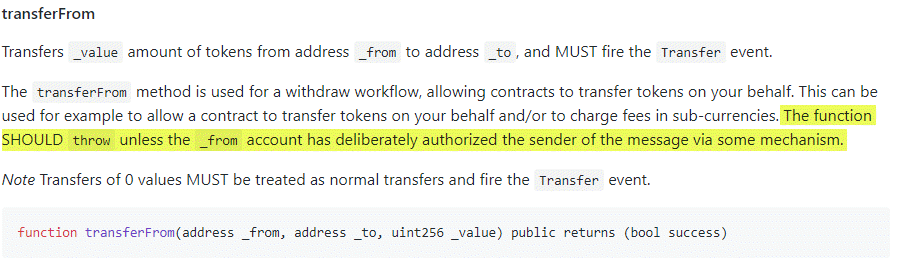
\includegraphics[width=1.0\linewidth]{figures/multiple_withdrawal_30.png}
	\caption{ERC20 \texttt{transferFrom} method definition that emphasizes on throwing an exception when the spender is not authorized to move tokens.\label{fig:standard}}
\end{figure}

\begin{figure}[t]
	\centering
	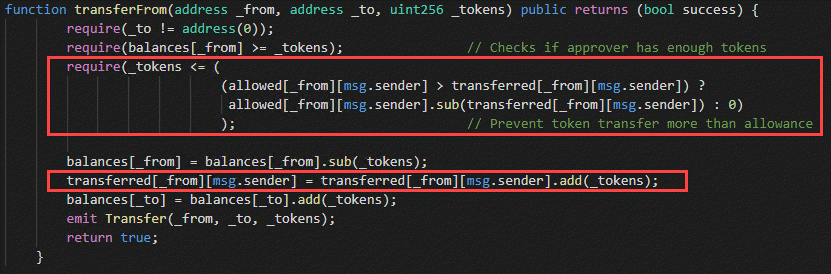
\includegraphics[width=1.0\linewidth]{figures/multiple_withdrawal_31.png}
	\caption{Securing \texttt{transferFrom} method instead of \texttt{approve} method can mitigate the attack by preventing more token transfer than allowed.\label{fig:transfer2}}
\end{figure}

% Based on ERC20 specifications, "approve functions allows \texttt{\_spender} to withdraw from your account multiple times, up to the \texttt{\_value}". Therefore, spender must not be able to transfer more than allowed tokens. That being said, \texttt{transferFrom} method can prevent transferring of new tokens in case of already transferred tokens up to allowed amount. By comparing transferred tokens in \texttt{transferFrom} method, spender will be restricted to move solely the remaining tokens of his allowance. In case of trying to transfer more tokens than allowed, the transaction fails. For example, Alice's new transaction for increasing Bob allowance from 100 to 110, sets Bob allowance to 110 (\texttt{approve} method sets allowance regardless of transferred tokens). However, \texttt{transferFrom} method prevent the attack by not allowing Bob to transfer more than 10 tokens if he had already transferred 100 tokens. We implemented this approach in~\ref{sec:proposal2} and it mitigates the attack effectively.

As an alternative to Proposal 1, we can also consider securing the \texttt{transferFrom} method. As specified by the ERC20 standard (see figure~\ref{fig:standard}), the goal here is to prevent the spender from transferring more tokens than allowed. Based on this assumption, we should not rely solely on the allowance value in deciding whether to allow or prevent an approve and should also consider the number of transferred tokens, which requires new state as in Proposal 1. 

Our solution, which is compliant with a careful reading of ERC20, is to interpret allowance as a `global' or `lifetime' allowance value, instead of the amount allowed at the specific time of invocation. For example, say Alice approves Bob for 50 tokens, Bob transfers 50 tokens, Alice approves Bob for 30 (more) tokens, and Bob transfers 30 tokens. In our implementation, Alice would approve Bob for 50 tokens and he transfers 50 tokens. To approve Bob for 30 more tokens, she approves Bob for 80 tokens. He has already spent 50 of these 80 tokens so he will only be allowed to transfer an addition 30. Thus 80 is his lifetime allowance and 50 (kept internally) is the amount he has transferred. In a bit more detail, consider the following, which prevents multiple withdrawals by modifying the implementation of \texttt{transferFrom} but keeping \texttt{approve} untouched:

\begin{enumerate}
	\item Alice approvals Bob to transferring 100 tokens
	\item Alice broadcasts an approval of 70, decreasing Bob's allowance.
	\item Bob front-runs Alice’s transaction and transfers 100 tokens (remark: a legitimate transfer).
	\item Alice's transaction is confirmed and sets Bob allowance to 70 by the default \texttt{approve} method.
	\item Bob's noticed the new allowance and tries to move 70 additional tokens by broadcasting \texttt{transferFrom(\_Bob,70)}. 
	\item Since Bob has already transferred more than 70 tokens, his transaction fails and prevents multiple withdrawal. 
	\item In the end, Bob’s allowance is set at 70 and his transferred tokens are set at 100.
\end{enumerate}

\subsubsection*{Performance \& Discussion} Interpreting \texttt{allowance} as a lifetime allowance is completely in accordance with the ERC20 standard (see figure~\ref{fig:standard}). In our solution, there is no relation between allowance (\texttt{allowed[\_from][msg.sender]}) and transferred tokens (\texttt{transferred[\_from][msg.sender]}). The first variable shows lifetime transferable tokens by a spender and can be changed independently of the transferred tokens (\ie \texttt{approve} method does not check transferred tokens). If Bob has not already transferred that many tokens, he would be able to transfer the difference of it. 

Our token is implemented as TKNv3\footnote{https://rinkeby.etherscan.io/address/0x5d148c948c01e1a61e280c8 b2ac39fd49ee6d9c6} on Rinkeby test network and it passes compatibility checks by transferring tokens between standard wallets. In terms of gas consumption, its \texttt{transferFrom} function needs at about 37\% more gas than standard \texttt{transferFrom} implementation. We believe this is acceptable for having a secure ERC20 token.

